\documentclass[letterpaper,12pt,twoside,]{pinp}

%% Some pieces required from the pandoc template
\providecommand{\tightlist}{%
  \setlength{\itemsep}{0pt}\setlength{\parskip}{0pt}}

% Use the lineno option to display guide line numbers if required.
% Note that the use of elements such as single-column equations
% may affect the guide line number alignment.

\usepackage[T1]{fontenc}
\usepackage[utf8]{inputenc}
\usepackage{longtable}

% pinp change: the geometry package layout settings need to be set here, not in pinp.cls
\geometry{layoutsize={0.95588\paperwidth,0.98864\paperheight},%
  layouthoffset=0.02206\paperwidth, layoutvoffset=0.00568\paperheight}

\definecolor{pinpblue}{HTML}{185FAF}  % imagecolorpicker on blue for new R logo
\definecolor{pnasbluetext}{RGB}{101,0,0} %



\title{Exercise - How Deep is the Ocean? September 16, 2020.}

\author[a]{EPIB607 - Inferential Statistics}

  \affil[a]{Fall 2020, McGill University}

\setcounter{secnumdepth}{5}

% Please give the surname of the lead author for the running footer
\leadauthor{Bhatnagar}

% Keywords are not mandatory, but authors are strongly encouraged to provide them. If provided, please include two to five keywords, separated by the pipe symbol, e.g:
 \keywords{  Sampling distribution |  Means |  Proportions |  Standard error |  Standard deviation |  Parameter |  Statistic  }  

\begin{abstract}
This in-class exercise will introduce you to sampling distributions for
means and proportions.
\end{abstract}

\dates{This version was compiled on \today} 

% initially we use doi so keep for backwards compatibility
% new name is doi_footer

\pinpfootercontents{Exercise: Sampling Distributions for Means and Proportions}

\begin{document}

% Optional adjustment to line up main text (after abstract) of first page with line numbers, when using both lineno and twocolumn options.
% You should only change this length when you've finalised the article contents.
\verticaladjustment{-2pt}

\maketitle
\thispagestyle{firststyle}
\ifthenelse{\boolean{shortarticle}}{\ifthenelse{\boolean{singlecolumn}}{\abscontentformatted}{\abscontent}}{}

% If your first paragraph (i.e. with the \dropcap) contains a list environment (quote, quotation, theorem, definition, enumerate, itemize...), the line after the list may have some extra indentation. If this is the case, add \parshape=0 to the end of the list environment.


\hypertarget{what-percentage-of-the-worlds-surface-is-covered-by-water}{%
\section{What percentage of the world's surface is covered by
water?}\label{what-percentage-of-the-worlds-surface-is-covered-by-water}}

The data provided by the
\href{https://topex.ucsd.edu/cgi-bin/get_srtm30.cgi}{Scripps Institution
of Oceanography} can provide an answer, but some work is required on
your part. James Hanley (JH) has randomly sampled \(n=5\) and \(n=20\)
latitudes and longitudes for every student in the class. This document
contains unique latitudes and longitudes for

\begin{ShadedResult}
\begin{verbatim}
character(0)
\end{verbatim}
\end{ShadedResult}

and was sent in an email (using the
\href{https://cran.r-project.org/package=gmailr}{gmailr} package) as a
pdf attachment to the following address:

\begin{ShadedResult}
\begin{verbatim}
[1] "sahir.bhatnagar@mcgill.ca"
\end{verbatim}
\end{ShadedResult}

\hypertarget{a-sample-of-5}{%
\subsection*{A sample of 5}\label{a-sample-of-5}}
\addcontentsline{toc}{subsection}{A sample of 5}

\begin{ShadedResult}
\begin{verbatim}
Latitude.n.5 <- c(-2.948,-9.253,45.707,10.364,-58.889)
\end{verbatim}
\end{ShadedResult}
\begin{ShadedResult}
\begin{verbatim}
Longitude.n.5 <- c(139.137,-120.824,162.652,-104.022,-50.878)
\end{verbatim}
\end{ShadedResult}

\hypertarget{a-sample-of-20}{%
\subsection*{A sample of 20}\label{a-sample-of-20}}
\addcontentsline{toc}{subsection}{A sample of 20}

\begin{ShadedResult}
\begin{verbatim}
Latitude.n.20 <- c(37.691,27.663,-43.884,49.942,-60.919,-1.777,55.886,-5.954,52.289,-46.256,
-19.198,-44.583,-25.221,-61.067,18.672,40.195,-46.15,-3.687,-45.854,-49.987)
\end{verbatim}
\end{ShadedResult}
\begin{ShadedResult}
\begin{verbatim}
Longitude.n.20 <- c(-176.024,-6.092,-142.938,73.052,72.392,-68.198,-12.536,77.866,2.048,70.171,
-150.271,-71.325,-159.891,143.669,-20.018,-60.647,59.549,-122.67,138.459,57.433)
\end{verbatim}
\end{ShadedResult}

\hypertarget{determine-the-proportion-of-water-from-the-sample-of-5}{%
\subsection{Determine the proportion of water from the sample of
5}\label{determine-the-proportion-of-water-from-the-sample-of-5}}

\begin{enumerate}
\def\labelenumi{\arabic{enumi}.}
\tightlist
\item
  Using the sample of 5, manually enter the latitudes and longitudes in
  \href{https://www.google.com/maps}{Google maps} and record if you land
  on water or land. Figure\ref{maps} shows how to enter them.
\end{enumerate}

\begin{figure}[H]
  \begin{center}
    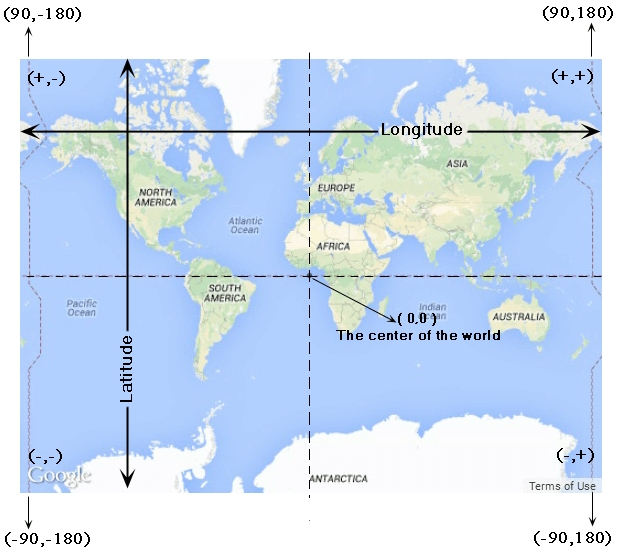
\includegraphics[scale=0.40]{lat-long.png} 
  \end{center}
  \caption{Latitude and longitude in Google maps. Latitudes range from (-90,90) and longitudes range from (-180, 180). Latitude is entered first followed by longitude and separated by a comma.}\label{maps}
\end{figure}

\begin{enumerate}
\def\labelenumi{\arabic{enumi}.}
\setcounter{enumi}{1}
\tightlist
\item
  In \texttt{R}, store your results in a binary vector of length 5. For
  example, if your sample landed on water 3 times out of 5, then you
  would enter the following in \texttt{R} (1 for water and 0 for land):
\end{enumerate}

\begin{ShadedResult}
\begin{verbatim}
landed_in_water <- c(1,1,1,0,0)
\end{verbatim}
\end{ShadedResult}

\begin{enumerate}
\def\labelenumi{\arabic{enumi}.}
\setcounter{enumi}{2}
\item
  Using \texttt{R}, estimate the percentage of the world's surface
  covered by water from your sample of 5. This can be done by simply
  taking the mean of the binary vector created in Step 2:
  \texttt{mean(landed\_in\_water)}.
\item
  Enter your estimate in this
  \href{https://docs.google.com/spreadsheets/d/1Mnxeq9nQcTdQycZ7S_62fYFiNC5_a3fibsyodzfwO58/edit?usp=sharing}{Google
  sheet} next to your name and in the column titled
  \texttt{PropnW.5.locations}.
\end{enumerate}

\hypertarget{determine-the-proportion-of-water-from-the-sample-of-20}{%
\subsection{Determine the proportion of water from the sample of
20}\label{determine-the-proportion-of-water-from-the-sample-of-20}}

\begin{enumerate}
\def\labelenumi{\arabic{enumi}.}
\tightlist
\item
  Repeat the above steps for the sample of 20. \textbf{Before you do},
  take a moment to think about how tedious a process it can be to
  manually enter 20 latitudes and longitudes into Google maps. SB hope
  you can appreciate the parallels between this toy exercise and that of
  collecting data for your research projects, i.e., it becomes
  increasingly difficult (effort and money!) to collect more and more
  samples.
\end{enumerate}

Now that you appreciate the amount of work it takes to estimate the
proportion of water from 20 samples, SB thinks it is sufficient for you
to use some automatic procedures to complete this task, which are
further described in step 2.

\begin{enumerate}
\def\labelenumi{\arabic{enumi}.}
\setcounter{enumi}{1}
\tightlist
\item
  Create an \texttt{R} script and copy the following index vector into
  it:
\end{enumerate}

\begin{ShadedResult}
\begin{verbatim}
index.n.20 <- c(2156,2157,2158,2159,2160,2161,2162,2163,2164,2165,
2166,2167,2168,2169,2170,2171,2172,2173,2174,2175)
\end{verbatim}
\end{ShadedResult}

\begin{enumerate}
\def\labelenumi{\arabic{enumi}.}
\setcounter{enumi}{2}
\tightlist
\item
  Load a function into your \texttt{R} session that JH and SB created to
  automate the process using the following command:
\end{enumerate}

\begin{Shaded}
\begin{Highlighting}[]
\KeywordTok{source}\NormalTok{(}\StringTok{"https://github.com/sahirbhatnagar/EPIB607/raw/gh-pages/resources/assets/labs/003-ocean-depths/automate_water_task.R"}\NormalTok{)}
\end{Highlighting}
\end{Shaded}

\begin{enumerate}
\def\labelenumi{\arabic{enumi}.}
\setcounter{enumi}{3}
\tightlist
\item
  Now that the function \texttt{automate\_water\_task} has been loaded
  into your environment, you can use it to automatically determine which
  of the locations in your sample of 20 are on water. This function
  requires the unique index vector shown in Step 2 above as input and
  returns a binary vector of length 20 (1 for water, 0 for land). You
  can call the function as follows in \texttt{R}:
\end{enumerate}

\begin{Shaded}
\begin{Highlighting}[]
\NormalTok{landed_in_water <-}\StringTok{ }\KeywordTok{automate_water_task}\NormalTok{(}\DataTypeTok{index =}\NormalTok{ index.n}\FloatTok{.20}\NormalTok{)}
\end{Highlighting}
\end{Shaded}

As before, enter your estimate of the proportion of the earth's surface
covered by water in this
\href{https://docs.google.com/spreadsheets/d/1Mnxeq9nQcTdQycZ7S_62fYFiNC5_a3fibsyodzfwO58/edit?usp=sharing}{Google
sheet} next to your name, but in the column titled
\texttt{PropnW.20.locations}.

\hypertarget{what-is-the-average-depth-of-the-ocean}{%
\section{What is the average depth of the
ocean?}\label{what-is-the-average-depth-of-the-ocean}}

We will now turn to estimating the average depth of the ocean. You will
again make use of the \texttt{automate\_water\_task} function.

\hypertarget{determine-the-average-depth-of-the-ocean-from-the-sample-of-5-and-20}{%
\subsection{Determine the average depth of the ocean from the sample of
5 and
20}\label{determine-the-average-depth-of-the-ocean-from-the-sample-of-5-and-20}}

\begin{enumerate}
\def\labelenumi{\arabic{enumi}.}
\tightlist
\item
  In the same \texttt{R} script as before, copy the following index
  vector into it:
\end{enumerate}

\begin{ShadedResult}
\begin{verbatim}
index.n.5 <- c(2151,2152,2153,2154,2155)
\end{verbatim}
\end{ShadedResult}

\begin{enumerate}
\def\labelenumi{\arabic{enumi}.}
\setcounter{enumi}{1}
\tightlist
\item
  Use the \texttt{automate\_water\_task} function to get a sample of 5
  depths. Note: some of the returned samples will not correspond to the
  same latitudes and longitudes provided to you earlier. This is because
  we need to restict our sample to locations on water only in order to
  estimate the mean depth of the ocean. Here we show some example code
  and its output. You need to specify the \texttt{type} and
  \texttt{student\_id} argument:
\end{enumerate}

\begin{Shaded}
\begin{Highlighting}[]
\CommentTok{# be sure to provide your own student id}
\NormalTok{depths.n}\FloatTok{.5}\NormalTok{ <-}\StringTok{ }\KeywordTok{automate_water_task}\NormalTok{(}\DataTypeTok{index =}\NormalTok{ index.n}\FloatTok{.5}\NormalTok{, }\DataTypeTok{student_id =} \DecValTok{222333444}\NormalTok{, }\DataTypeTok{type =} \StringTok{"depth"}\NormalTok{)}
\end{Highlighting}
\end{Shaded}

\newpage

The \texttt{alt} column gives the depth in meters:

\begin{longtable}[]{@{}lrrrrr@{}}
\toprule
& X & lon & lat & alt & water\tabularnewline
\midrule
\endhead
3 & 3 & -134.382568 & 37.74272 & 5028 & 1\tabularnewline
4 & 4 & -23.623316 & -12.23716 & 5358 & 1\tabularnewline
43091 & 43091 & -41.047879 & 47.44291 & 4585 & 1\tabularnewline
25933 & 25933 & 1.778625 & 50.96857 & 10 & 1\tabularnewline
14723 & 14723 & -53.129054 & 44.92232 & 68 & 1\tabularnewline
\bottomrule
\end{longtable}

\begin{enumerate}
\def\labelenumi{\arabic{enumi}.}
\setcounter{enumi}{2}
\item
  Repeat step 2 for a sample of 20 using the \texttt{index.n.20} vector
  specified above.
\item
  Calculate an estimate of the mean depth of the ocean from your samples
  of 5 and 20 using the \texttt{mean} function, e.g.,
  \texttt{mean(depths.n.5\$alt)}.
\item
  Enter your estimates of the mean depth of the ocean from your samples
  of 5 and 20 in this
  \href{https://docs.google.com/spreadsheets/d/1Mnxeq9nQcTdQycZ7S_62fYFiNC5_a3fibsyodzfwO58/edit?usp=sharing}{Google
  sheet} next to your name, in the columns titled \texttt{Mean.5.depths}
  and \texttt{Mean.20.depths}, respectively.
\end{enumerate}

\hypertarget{plot-the-sampling-distribution-of-the-proportion-and-mean}{%
\section{Plot the sampling distribution of the proportion and
mean}\label{plot-the-sampling-distribution-of-the-proportion-and-mean}}

It is now time to plot the sampling distributions of the proportions and
means. Once everyone has filled in the
\href{https://docs.google.com/spreadsheets/d/1Mnxeq9nQcTdQycZ7S_62fYFiNC5_a3fibsyodzfwO58/edit?usp=sharing}{Google
sheet}, export the sheet as a \texttt{.csv} file by clicking on
\texttt{File\ -\/-\textgreater{}\ Download\ as\ -\/-\textgreater{}\ Comma-separated\ values\ (.csv,\ current\ sheet)}.

\begin{enumerate}
\def\labelenumi{\arabic{enumi}.}
\tightlist
\item
  Read in the data:
\end{enumerate}

\begin{Shaded}
\begin{Highlighting}[]
\CommentTok{# read in the results from the Google sheet }
\NormalTok{water_results <-}\StringTok{ }\KeywordTok{read.csv}\NormalTok{(}\StringTok{"EPIB607_FALL2020_water_exercise - water.csv"}\NormalTok{, }\DataTypeTok{as.is=}\OtherTok{TRUE}\NormalTok{)}
\NormalTok{water_results <-}\StringTok{ }\NormalTok{water_results[,}\DecValTok{1}\OperatorTok{:}\DecValTok{6}\NormalTok{]}
\NormalTok{water_results <-}\StringTok{ }\NormalTok{water_results[}\KeywordTok{complete.cases}\NormalTok{(water_results), ]}

\CommentTok{# count the number of students who provided a mean and proportion}
\NormalTok{N.r <-}\StringTok{ }\KeywordTok{nrow}\NormalTok{(water_results)}
\end{Highlighting}
\end{Shaded}

\begin{enumerate}
\def\labelenumi{\arabic{enumi}.}
\setcounter{enumi}{1}
\tightlist
\item
  Plot the students' estimates of the proportion covered by water for
  samples of size 5. You may use the following code or run your own:
\end{enumerate}

\begin{Shaded}
\begin{Highlighting}[]
\KeywordTok{plot}\NormalTok{(}\KeywordTok{table}\NormalTok{(water_results[,}\StringTok{"PropnW.5.locations"}\NormalTok{]), }
     \DataTypeTok{xlim =} \KeywordTok{c}\NormalTok{(}\DecValTok{0}\NormalTok{,}\DecValTok{1}\NormalTok{),}
     \DataTypeTok{xlab =} \StringTok{"Students' Estimates of Proportion Covered by Water"}\NormalTok{,}
     \DataTypeTok{main =} \StringTok{"n = 5"}\NormalTok{, }
     \DataTypeTok{ylim =} \KeywordTok{c}\NormalTok{(}\DecValTok{0}\NormalTok{, N.r}\OperatorTok{/}\FloatTok{1.5}\NormalTok{), }
     \DataTypeTok{ylab =} \StringTok{"Frequency"}\NormalTok{)}
\end{Highlighting}
\end{Shaded}

\begin{enumerate}
\def\labelenumi{\alph{enumi})}
\tightlist
\item
  Comment on this graph. Does this shape look sensible to you?
\end{enumerate}

\begin{enumerate}
\def\labelenumi{\arabic{enumi}.}
\setcounter{enumi}{2}
\tightlist
\item
  Now plot the students' estimates of the mean depth of the ocean for
  samples of size 5. You may use the following code or run your own:
\end{enumerate}

\begin{Shaded}
\begin{Highlighting}[]
\NormalTok{d.BREAKS <-}\StringTok{ }\KeywordTok{seq}\NormalTok{(}\DecValTok{1000}\NormalTok{,}\DecValTok{6000}\NormalTok{,}\DecValTok{500}\NormalTok{)}
\KeywordTok{hist}\NormalTok{(water_results[,}\StringTok{"Mean.5.depths"}\NormalTok{], }
     \DataTypeTok{xlim =} \KeywordTok{c}\NormalTok{(}\DecValTok{0}\NormalTok{,}\DecValTok{6000}\NormalTok{),}
     \DataTypeTok{ylim =} \KeywordTok{c}\NormalTok{(}\DecValTok{0}\NormalTok{, N.r}\OperatorTok{/}\FloatTok{1.5}\NormalTok{), }
     \DataTypeTok{breaks =}\NormalTok{ d.BREAKS,}
     \DataTypeTok{xlab =} \StringTok{"Students' Estimates of Mean Ocean Depth (m)"}\NormalTok{,}
     \DataTypeTok{main =} \StringTok{"n = 5"}\NormalTok{)}
\end{Highlighting}
\end{Shaded}

\begin{enumerate}
\def\labelenumi{\alph{enumi})}
\tightlist
\item
  Calculate the mean and the standard error of the mean depth for
  samples of size 5
\item
  Comment on this graph (e.g.~range, variability)
\end{enumerate}

\begin{enumerate}
\def\labelenumi{\arabic{enumi}.}
\setcounter{enumi}{3}
\tightlist
\item
  Repeat Steps 2 and 3 for samples of size 20.
\end{enumerate}

\begin{enumerate}
\def\labelenumi{\alph{enumi})}
\tightlist
\item
  Compare the two graphs for proportions, and the two graphs for means.
  What do you notice? You might find it helpful to overlay the
  distributions on the sample plot. You may use the following code or
  run your own:
\end{enumerate}

\begin{Shaded}
\begin{Highlighting}[]
\KeywordTok{library}\NormalTok{(mosaic)}
\KeywordTok{library}\NormalTok{(tidyr)}

\CommentTok{# first 'melt' the data to get it in plotting form}
\NormalTok{m.melt <-}\StringTok{ }\NormalTok{water_results }\OperatorTok\StringTok{ }\NormalTok{tidyr}\OperatorTok{::}\KeywordTok{gather}\NormalTok{(}\DataTypeTok{key =} \StringTok{"type"}\NormalTok{, }\DataTypeTok{value =} \StringTok{"value"}\NormalTok{, }\OperatorTok{-}\NormalTok{X., }\OperatorTok{-}\NormalTok{student)}

\CommentTok{# subset for means}
\NormalTok{m.melt.means <-}\StringTok{ }\KeywordTok{subset}\NormalTok{(m.melt, type }\OperatorTok\StringTok{ }\KeywordTok{c}\NormalTok{(}\StringTok{"Mean.20.depths"}\NormalTok{,}\StringTok{"Mean.5.depths"}\NormalTok{))}

\CommentTok{# plot for means}
\KeywordTok{gf_density}\NormalTok{(}\OperatorTok{~}\StringTok{ }\NormalTok{value, }\DataTypeTok{data =}\NormalTok{ m.melt.means, }\DataTypeTok{fill =} \OperatorTok{~}\StringTok{ }\NormalTok{type) }\OperatorTok{+}\StringTok{ }\KeywordTok{theme_bw}\NormalTok{()}

\CommentTok{# subset for proportions}
\NormalTok{m.melt.props <-}\StringTok{ }\KeywordTok{subset}\NormalTok{(m.melt, type }\OperatorTok\StringTok{ }\KeywordTok{c}\NormalTok{(}\StringTok{"PropnW.20.locations"}\NormalTok{,}\StringTok{"PropnW.5.locations"}\NormalTok{))}

\CommentTok{# plot for proportions}
\KeywordTok{gf_histogram}\NormalTok{(}\OperatorTok{~}\StringTok{ }\NormalTok{value, }\DataTypeTok{data =}\NormalTok{ m.melt.props, }\DataTypeTok{fill =} \OperatorTok{~}\StringTok{ }\NormalTok{type, }\DataTypeTok{position =} \StringTok{"dodge"}\NormalTok{) }\OperatorTok{+}\StringTok{ }\KeywordTok{theme_bw}\NormalTok{()}
\end{Highlighting}
\end{Shaded}

%\showmatmethods


\bibliography{pinp}
\bibliographystyle{jss}



\end{document}

